\section{Charge-State Transition Levels and the $U$ Parameter}

\paragraph{The formation energy as a function of the Fermi level.}
\textcolor{red}{Here, $E^f_0[X^q]$ denotes the formation energy at $E_F=0$,
with $E_F$ measured from the valence-band maximum (VBM).}
The formation energy of Section~1 depends on the Fermi level through the
term $qE_F$ only,
\begin{equation*}
    E^f[X^q]=E^f_0[X^q]+qE_F.
\end{equation*}
In a plot against $E_F$, each charge state is a straight line with the slope
$q$. At a given $E_F$, the defect takes the charge state with the lowest
formation energy, so the stable charge state follows the
\textcolor{blue}{lower envelope} of the lines (red in
Fig.~\ref{fig:transition-levels}). The Fermi level ranges from the VBM to the
conduction-band minimum (CBM).

\paragraph{Charge-state transition levels.}
The \textcolor{blue}{charge-state transition level} $\varepsilon(q/q')$ is the
Fermi level at which the charge states $q$ and $q'$ have equal formation
energies. Equating the two lines gives
\begin{equation}
    \boxed{\varepsilon(q/q')=\frac{E^f_0[X^{q'}]-E^f_0[X^q]}{q-q'}.}
\end{equation}
Below $\varepsilon(q/q')$, the more positive charge state is stable, and
above $\varepsilon(q/q')$, the more negative one is stable. The transition
levels are the kinks of the lower envelope.

\paragraph{The stability window of a charge state.}
Three consecutive charge states $q+1$, $q$ and $q-1$ have two transition
levels, $\varepsilon(q+1/q)=E^f_0[X^q]-E^f_0[X^{q+1}]$ and
$\varepsilon(q/q-1)=E^f_0[X^{q-1}]-E^f_0[X^q]$. The charge state $q$ is
stable only for Fermi levels between the two. The width of this window
defines the \textcolor{blue}{$U$ parameter},
\begin{equation}
    \boxed{U\equiv\varepsilon(q/q-1)-\varepsilon(q+1/q)
    =E^f[X^{q+1}]+E^f[X^{q-1}]-2E^f[X^q].}
\end{equation}
The terms in $E_F$ cancel, because $(q+1)+(q-1)-2q=0$, so $U$ does not depend
on the Fermi level.

\paragraph{$U$ as a reaction energy.}
The right-hand side of the definition is the energy change of the
\textcolor{blue}{disproportionation reaction}
\begin{equation*}
    2X^q\to X^{q+1}+X^{q-1},
\end{equation*}
in which one defect passes an electron to another. The electron does not
reach the reservoir, which explains why $E_F$ drops out.

\paragraph{The sign of $U$.}
A second electron on the same defect feels the Coulomb repulsion of the
first, which favors $U>0$. The charge state $q$ is then stable in a window of
width $U$ (Fig.~\ref{fig:transition-levels}a). The lattice around the defect
can relax differently in each charge state, and a large relaxation can
outweigh the repulsion, so that $U<0$. The disproportionation then releases
energy, the line of the charge state $q$ lies above the crossing of the lines
$q+1$ and $q-1$ for every $E_F$, and the defect changes directly from $q+1$
to $q-1$ at the level $\varepsilon(q+1/q-1)$
(Fig.~\ref{fig:transition-levels}b). The vacancy in silicon is an example,
with an unstable $V^+$.

\paragraph{More charge states.}
With more than three charge states, the lower envelope selects the stable
ones in order of decreasing charge from the VBM to the CBM. Each charge state
that appears has a window of its own width, and a charge state with a
negative $U$ drops out, so that the envelope jumps by two units of slope at a
single kink (Fig.~\ref{fig:transition-levels}c).

\begin{figure}[htbp]
\centering
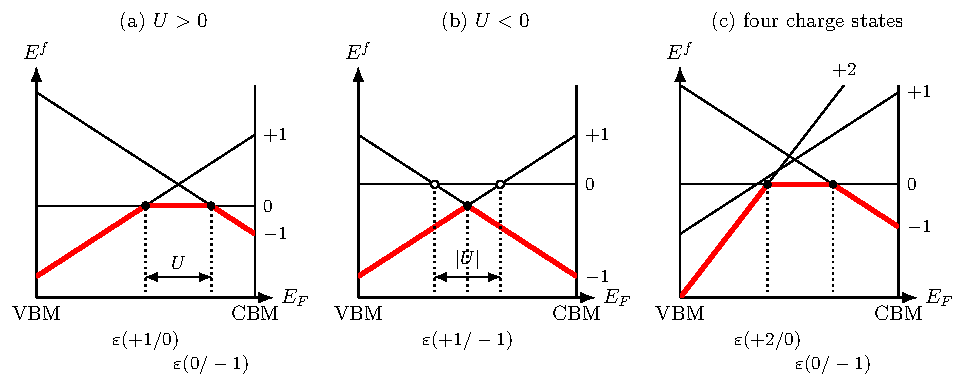
\includegraphics{figures/transition-levels}
\caption{Formation energy against the Fermi level for three model defects,
with the lower envelope in red. (a) Charge states $+1$, $0$ and $-1$ with
$U>0$ and a window for the neutral state. (b) The same charge states with
$U<0$. Open circles: crossings with the neutral line above the envelope. (c)
Charge states $+2$, $+1$, $0$ and $-1$, with the state $+1$ skipped and a
direct level $\varepsilon(+2/0)$.}
\label{fig:transition-levels}
\end{figure}
